% Foliensatz: "AFu-Kurs nach DJ4UF" von DK0TU, Amateurfunkgruppe der TU Berlin
% Lizenz: CC BY-NC-SA 3.0 de (http://creativecommons.org/licenses/by-nc-sa/3.0/de/)
% Autor: Martin Deutschmann
% Korrekturen: Lars Weiler <dc4lw@darc.de>, Hendrik Boerma

\documentclass[aspectratio=169]{beamer}

\usepackage[ngerman]{babel} % deutsche Worttrennung etc.
\usepackage[utf8]{inputenc} % UTF8 Text

\usepackage[super, comma, numbers, square, sort]{natbib}

\usepackage{hyperref}       % Hyperref Package für bessere Referenzen (todo)
\hypersetup{
	colorlinks=false,       %   false: boxed links; true: colored links
    %linkcolor=white,       %   color of internal links (change box color with linkbordercolor)
    citecolor=red,          %   color of links to bibliography
    filecolor=white,        %   color of file links
    urlcolor=blue           %   color of external links
}

\usepackage{multirow}
\usepackage{wasysym}  % Math Symbols like \permil
%\usepackage{colortbl}
%\usepackage{subscript}
%\usepackage{caption}
%\usepackage{setspace}
%\usepackage{xcolor}        % benutze CodeListe

% Footnote
%\usepackage{hanging}
%
%\setbeamertemplate{footnote}{%
%  \hangpara{2em}{1}%
%  \makebox[2em][l]{\insertfootnotemark}\footnotesize\insertfootnotetext\par%
%}


%\usepackage{pgf}
%\usepackage{tikz}
%\usetikzlibrary{arrows,automata}
%\usetikzlibrary{positioning}
%
%\tikzset{
%    state/.style={
%           rectangle,
%           rounded corners,
%           draw=black, very thick,
%           minimum height=2em,
%           minimum width=2pt,
%           inner sep=2pt,
%           text centered,
%           },
%}

%\usepackage{listings}
%\lstset{basicstyle=\small, numberstyle=\tiny, extendedchars=true, numbers=left, numbersep=5pt}
%\lstset{showtabs=false, showspaces=false, showstringspaces=false}
%%\lstset{backgroundcolor=\color{white!75!lightgray}, , frame=single}
%%\lstset{backgroundcolor=\color{white}}
%%\lstset{backgroundcolor=none}
%\lstset{keywordstyle=\color{blue!50!gray},  identifierstyle=\color{black}}
%\lstset{commentstyle=\color{green!50!gray}, stringstyle=\color{red!50!gray}}
%\lstset{language=C, fontadjust=true, tabsize=2, breaklines=true}
%\lstset{backgroundcolor=\color{white!75!lightgray}, caption=\lstname, frame=single}
%\lstset{emphstyle=\color{black}\fbox}
%
%% Keine "Listing:"-Caption
%\captionsetup{labelformat=empty,labelsep=none}
%
%% für mathematische Umgebungen
%\usepackage{amsmath,amsfonts,amssymb}
%
%\lstdefinestyle{Bash}{
%language=Bash,
%frame=single,
%rulecolor=\color{black},
%backgroundcolor=\color{gray!50},
%keywordstyle=\color{black},
%identifierstyle=,
%commentstyle=\color{black},
%stringstyle=\color{magenta!65!white},
%showstringspaces=false,
%basicstyle=\footnotesize\ttfamily\color{black},
%numbers=none,
%breaklines=true,
%captionpos=b
%}

%\usepackage{listings}
%
%\lstdefinestyle{basic}{
%    captionpos=t,%
%    basicstyle=\footnotesize\ttfamily,%
%    numberstyle=\tiny,%
%    numbers=left,%
%    stepnumber=1,%
%    frame=single,%
%    showspaces=false,%
%    showstringspaces=false,%
%    showtabs=false,%
%    %
%    keywordstyle=\color{blue},%
%    identifierstyle=,%
%    commentstyle=\color{gray},%
%    stringstyle=\color{magenta}%
%}



% fließende Boxen haben keinen Abstand
%\fboxsep0mm

% inkludiere Creative Commons Helper
%%%%%%%%%%%%%%%%%%%%%%%%%%%%%%%%%%%%%%%%%%%%%%%%%%%%%%%%%%%%%%%%
%% ccBeamer 0.1, 2007-07-02                                   %%
%% Written by Sebastian Pipping <webmaster@hartwork.org>      %%
%% ---------------------------------------------------------- %%
%% Licensed under Creative Commons Attribution-ShareAlike 3.0 %%
%% http://creativecommons.org/licenses/by-sa/3.0/             %%
%%%%%%%%%%%%%%%%%%%%%%%%%%%%%%%%%%%%%%%%%%%%%%%%%%%%%%%%%%%%%%%%


%% Images
\newcommand{\CcImageBy}[1]{%
	
\includegraphics[scale=#1]{texdata/creative_commons/cc_by_30.pdf}%
}
\newcommand{\CcImageCc}[1]{%
	
\includegraphics[scale=#1]{texdata/creative_commons/cc_cc_30.pdf}%
}
\newcommand{\CcImageDevNations}[1]{%
	
\includegraphics[scale=#1]{texdata/creative_commons/cc_dev_nations_30.pdf}%
}
\newcommand{\CcImageNc}[1]{%
	
\includegraphics[scale=#1]{texdata/creative_commons/cc_nc_30.pdf}%
}
\newcommand{\CcImageNd}[1]{%
	
\includegraphics[scale=#1]{texdata/creative_commons/cc_nd_30.pdf}%
}
\newcommand{\CcImagePd}[1]{%
	
\includegraphics[scale=#1]{texdata/creative_commons/cc_pd_30.pdf}%
}
\newcommand{\CcImageSa}[1]{%
	
\includegraphics[scale=#1]{texdata/creative_commons/cc_sa_30.pdf}%
}
\newcommand{\CcImageSampling}[1]{%
	
\includegraphics[scale=#1]{texdata/creative_commons/cc_sampling_30.pdf}%
}
\newcommand{\CcImageSamplingPlus}[1]{%
	
\includegraphics[scale=#1]{texdata/creative_commons/cc_sampling_plus_30.pdf}%
}


%% Groups
\newcommand{\CcGroupBy}[2]{% zoom, gap
	\CcImageCc{#1}\hspace*{#2}\CcImageBy{#1}%
}
\newcommand{\CcGroupByNc}[2]{% zoom, gap
	\CcImageCc{#1}\hspace*{#2}\CcImageBy{#1}\hspace*{#2}\CcImageNc{#1}%
}
\newcommand{\CcGroupByNcNd}[2]{% zoom, gap
	\CcImageCc{#1}\hspace*{#2}\CcImageBy{#1}\hspace*{#2}\CcImageNc{#1}\hspace*{#2}\CcImageNd{#1}%
}
\newcommand{\CcGroupByNcSa}[2]{% zoom, gap
	\CcImageCc{#1}\hspace*{#2}\CcImageBy{#1}\hspace*{#2}\CcImageNc{#1}\hspace*{#2}\CcImageSa{#1}%
}
\newcommand{\CcGroupByNd}[2]{% zoom, gap
	\CcImageCc{#1}\hspace*{#2}\CcImageBy{#1}\hspace*{#2}\CcImageNd{#1}%
}
\newcommand{\CcGroupBySa}[2]{% zoom, gap
	\CcImageCc{#1}\hspace*{#2}\CcImageBy{#1}\hspace*{#2}\CcImageSa{#1}%
}
\newcommand{\CcGroupDevNations}[2]{% zoom, gap
	\CcImageCc{#1}\hspace*{#2}\CcImageDevNations{#1}%
}
\newcommand{\CcGroupNcSampling}[2]{% zoom, gap
	\CcImageCc{#1}\hspace*{#2}\CcImageNc{#1}\hspace*{#2}\CcImageSampling{#1}%
}
\newcommand{\CcGroupPd}[1]{% zoom
	\CcImagePd{#1}%
}
\newcommand{\CcGroupSampling}[1]{% zoom
	\CcImageSampling{#1}%
}
\newcommand{\CcGroupSamplingPlus}[1]{% zoom
	\CcImageSamplingPlus{#1}%
}


%% Text
\newcommand{\CcLongnameBy}{Attribution}
\newcommand{\CcLongnameByNc}{Attribution-NonCommercial}
\newcommand{\CcLongnameByNcNd}{Attribution-NoDerivs}
\newcommand{\CcLongnameByNcSa}{Attribution-NonCommercial-ShareAlike}
\newcommand{\CcLongnameByNd}{Attribution-NoDerivs}
\newcommand{\CcLongnameBySa}{Attribution-ShareAlike}

\newcommand{\CcNote}[1]{% longname
	This work is licensed under the \textit{Creative Commons #1 3.0 License}.%
}


% generelles Thema auswählen
\usetheme{Goettingen} %Berlin spart ohne Sidebar allerdings angenehm Platz
% AnnArbor | Antibes | Bergen | Berkeley | Berlin | Boadilla | boxes | CambridgeUS | Copenhagen | Darmstadt | default | Dresden | Frankfurt | Goettingen | Hannover | Ilmenau | JuanLesPins | Luebeck | Madrid | Malmoe | Marburg | Montpellier | PaloAlto | Pittsburgh | Rochester | Singapore | Szeged | Warsaw

% Farben wählen
\usecolortheme{beetle}
% beaver | beetle | crane | default | dolphin | dove | fly | lily | orchid | rose | seagull | seahorse | sidebartab | structure | whale | wolverine

% Setze alle Farben auf Grau und Weiß
%\definecolor{craneorange}{RGB}{64,64,64}
%\definecolor{craneblue}{RGB}{255,255,255}

% Schriftart wählen
\usefonttheme{default}
% default | professionalfonts | serif | structurebold | structureitalicserif | structuresmallcapsserif

% Innere Themen(Kopf-, Fuß-, Sidebar usw)
%\useinnertheme{default}
\useinnertheme{circles}
% default | inmargin | rectangles | rounded | circles

% Äußere Themen (Anordnung der inneren, grenzen der Folien etc.)
\useoutertheme{infolines}
% default | infolines | miniframes | shadow | sidebar | smoothbars | smoothtree | split | tree

% Deaktiviere Navigations-Symbole ({} -> leer)
\setbeamertemplate{navigation symbols}{}
%\setbeamertemplate{navigation symbols}{\large \ifnum \insertframenumber <10 0\fi\insertframenumber/\inserttotalframenumber\vspace*{0.2ex}}

% Zeige ein Hintergrundbild
\setbeamertemplate{background canvas}{
        \hspace*{-2.0cm}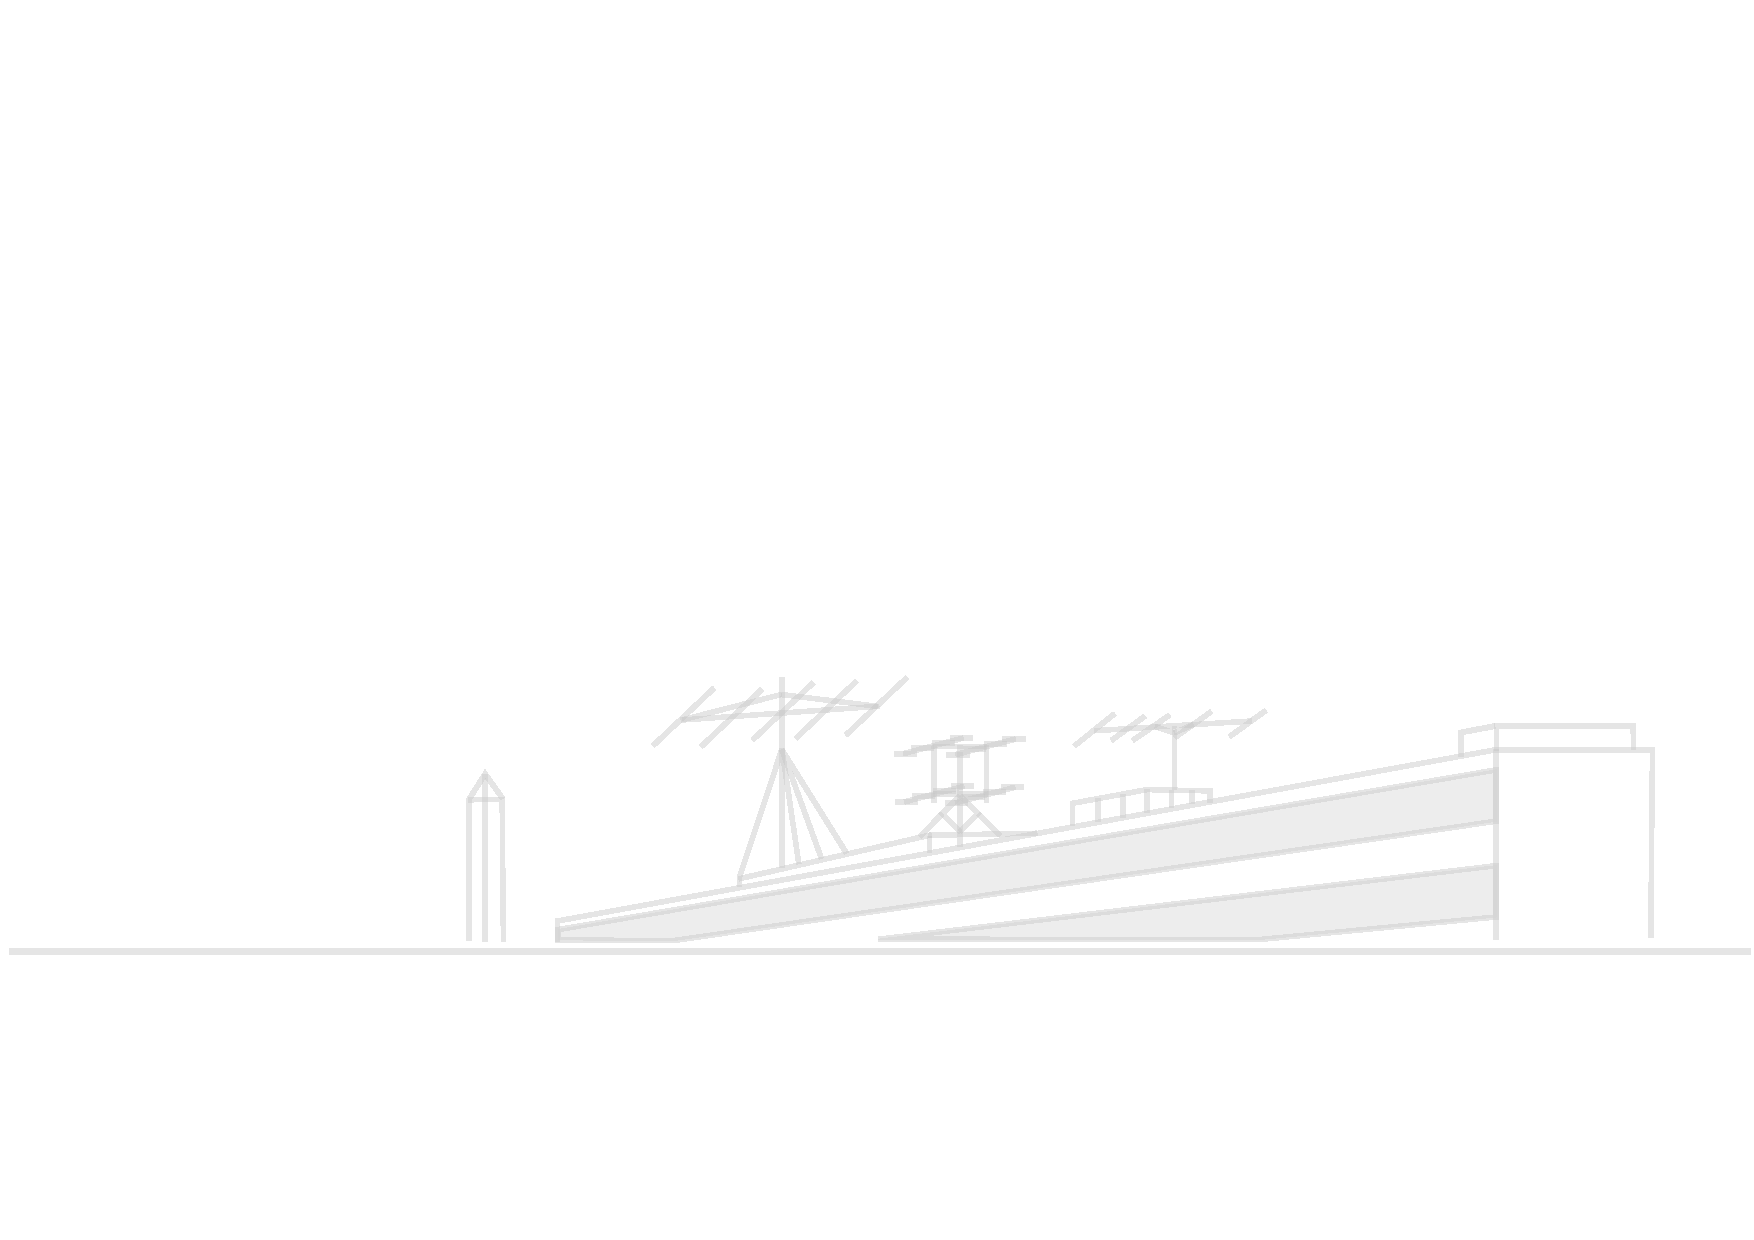
\includegraphics[width=17.8cm]{texdata/dk0tu_rooftop_background.pdf}
}

% Foliennummer einfügen
\setbeamertemplate{footline}[frame number]
%\setbeamertemplate{footline}{}

% Ändere das Zeichen vor jedem item
%\setbeamertemplate{itemize item}{\color{craneorange}$\blacktriangleright$}
%\setbeamertemplate{itemize subitem}{\color{craneorange}$\triangleright$}
%\setbeamertemplate{itemize subsubitem}{\color{craneorange}$\blacktriangleright$}

% Ändert die Blöcke 
\setbeamertemplate{blocks}[rounded][shadow=true]
% default | rounded [shadow=true|false]

%
% Eigene Kommandos
%

% Hack to get natbib and beamer working together. "The beamer user guide suggests
% that only the manual bibliography entry approach is supported"
% on some system it works out of the box, sometimes you need the hack :-(
% so check it --dl7bst
\ifdefined\newblock
    \relax
\else
    \newcommand{\newblock}{}
\fi

% \includedia command to generate png out of a dia file
% NEEDS installed dia and pdflatex option --shell-escape
\newcommand{\includedia}[1]{
    \immediate\write18{/usr/bin/dia #1.dia -e #1_diatmp.png -t png}
}

% RICHIG GROSSER FONT!
\newfont{\bigfont}{cmr10 at 144pt}
\newfont{\smallfont}{cmr10 at 8pt}

% Römische Ziffern
\makeatletter
\newcommand{\rmnum}[1]{\romannumeral #1}
\newcommand{\Rmnum}[1]{\expandafter\@slowromancap\romannumeral #1@}
\makeatother

% Schwarze Überschrift
%\setbeamercolor{frametitle}{fg=black}
%\setbeamercolor{title}{fg=black}

% Item- und Box-Farben
\definecolor{deepBlue}{HTML}{000066}
\setbeamercolor{itemize item}{fg=deepBlue}
\setbeamercolor{itemize subitem}{fg=deepBlue}
\setbeamercolor{description item}{fg=deepBlue}
\setbeamercolor{block title}{fg=deepBlue!100, bg=blue!15}
\setbeamercolor{block body}{fg=black, bg=blue!5}
\setbeamercolor{block title alerted}{fg=deepBlue, bg=red!75}
\setbeamercolor{block body alerted}{fg=black, bg=red!15}
\setbeamercolor*{block title example}{fg=blue!50, bg=blue!10}
\setbeamercolor*{block body example}{fg= blue, bg=blue!5}

%\setbeamercolor{section in head/foot}{parent=palette primary}
%\setbeamercolor{subsection in head/foot}{parent=palette secondary}
%\setbeamercolor{sidebar}{fg=darkblue,bg=yellow!90!orange}
%\setbeamercolor{title in sidebar}{fg=darkblue}
%\setbeamercolor{author in sidebar}{fg=darkblue}
%\setbeamercolor{section in sidebar}{fg=darkblue!10!black}
%\setbeamercolor{subsection in sidebar}{fg=darkblue!50!black}

% Titlepage Infos
\title{AFu-Kurs nach DJ4UF}
\author[DKØTU]{DKØTU\\ \footnotesize{Amateurfunkgruppe der TU Berlin}}
\institute[DKØTU]{\url{http://www.dk0tu.de} }

% PDF-Eigenschaften
\subject{DK0TU-Amateurfunkkurs nach DJ4UF}
\keywords{Amateurfunk Kurs HAM Radio Course CC-BY-NC-SA OpenSource TU Berlin DK0TU}

\subtitle{Technik Klasse E 05: \\
  Der Kondensator und seine Schaltungsarten \\[2em]}
\date{Stand 18.09.2017}
 \begin{document}

\begin{frame}
    \titlepage
    \vfill
    \begin{center}
        \ccbyncsaeu\\
        {\tiny This work is licensed under the \em{Creative Commons Attribution-NonCommercial-ShareAlike 3.0 License}.}\\[0.5ex]
         \tiny Amateurfunkgruppe der Technische Universität Berlin (AfuTUB), DKØTU
         %\includegraphics[scale=0.5]{img/DK0TU_Logo.pdf}
    \end{center}
\end{frame}


\section*{Einleitung}

\begin{frame}
  \frametitle{Einleitung / Kondensator}
  \begin{center}
    \Large{Wie sieht er aus?}\\
    \Large{Was tut der?}
  \end{center}
\end{frame}


\begin{frame}
  \frametitle{Einleitung / Kondensator}

  \begin{center}
    \begin{figure}
      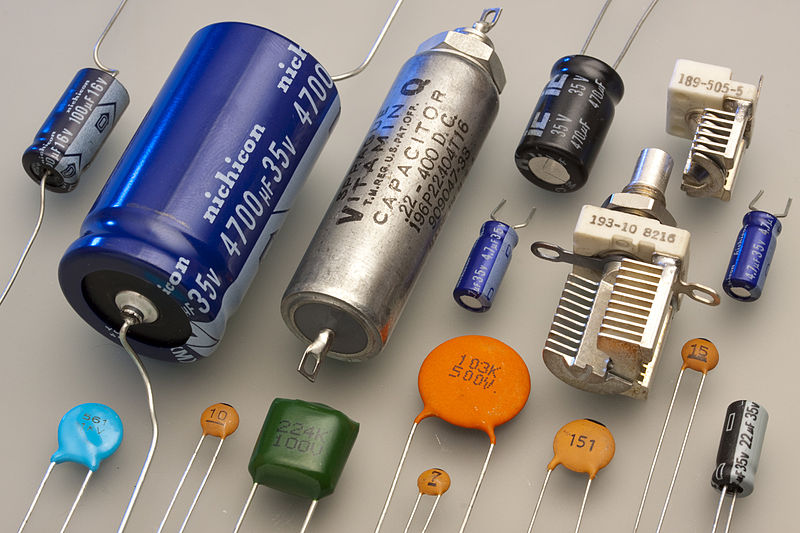
\includegraphics[width=0.7\textwidth,height=.75\textheight,keepaspectratio]{e05/Kondensator01.jpg}
      \attribcaption{Verschiedene Kondensatoren}{Eric Schrader}{https://commons.wikimedia.org/wiki/File:Capacitors_(7189597135).jpg}{\ccbysa}
    \end{figure}
  \end{center}


\end{frame}

\begin{frame}
  \frametitle{Einleitung / Kondensator}

  \begin{center}
    \begin{figure}
      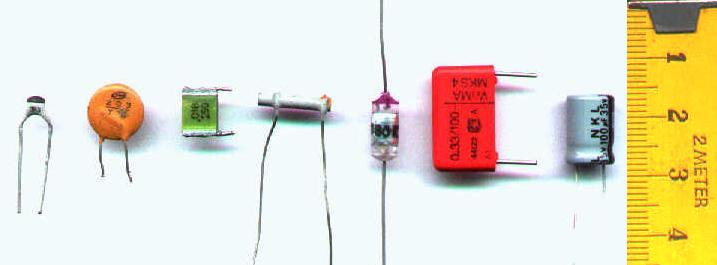
\includegraphics[width=0.8\textwidth,height=.75\textheight,keepaspectratio]{e05/Kondensator02.jpg}
      \attribcaption{Verschiedene kleine Kondensatoren}{Aka}{https://commons.wikimedia.org/wiki/File:Condensators.JPG}{\ccbysa}
    \end{figure}
  \end{center}
\end{frame}

\section*{Anwendungen}
\begin{frame}
  \frametitle{Diverse Anwendungsmöglichkeiten}
  \only<1>{Bisher kam ich ganz gut ohne Kondensatoren im Leben aus\ldots}
  \pause
  \begin{itemize}
    \item Energiespeicher
    \item Blitzlicht
    \item Signalentkopplung
    \item Filter
    \item Schwingkreise
    \item Glättung
    \item Entstörung
    \item Phasenkompensation
  \end{itemize}
\end{frame}


\section*{Kapazität}

\begin{frame}
  \frametitle{Kapazität}

  \begin{center}
    \begin{figure}
      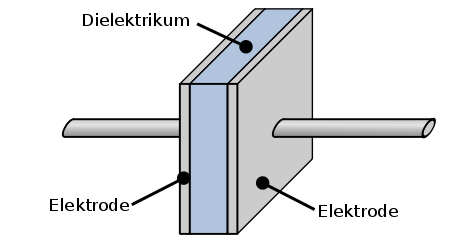
\includegraphics[width=0.8\textwidth,height=.75\textheight,keepaspectratio]{e05/c-aufbau.png}
      \attribcaption{Interner Aufbau eines Plattenkondensators}{Cepheiden}{https://de.wikipedia.org/wiki/Datei:Plate_Capacitor_DE.svg}{\ccbysa}
    \end{figure}
  \end{center}
\end{frame}

\section*{Gleich\-strom\-kreis}
\begin{frame}
  \frametitle{ein paar Formeln}
  \begin{block}{Berechnung eines Kondensators}
    \begin{center}
      \huge{$C = \frac{Q}{U}$} in $[C] = \frac{As}{V} = F$ (Farad)
    \end{center}
    Ladung des Kondensators im Verhältnis zur Spannung
  \end{block}
  \begin{block}{Berechnung eines Kondensators}
    \begin{center}
      \huge{$C= \varepsilon_{0} \cdot \varepsilon_{r} \cdot \cfrac{A}{d}$}\\
      \small{mit $\varepsilon_{0} = 0,885 \cdot 10^{-11} \frac{As}{Vm}$: Elektrische Feldkonstante\\
      $\varepsilon_{r}$: relative Dielektrizitätszahl}
    \end{center}
  \end{block}
  Sobald der Kondensator geladen ist, fließt kein Strom mehr.
\end{frame}

\section{Wechsel\-strom\-kreis}
\begin{frame}
  \frametitle{Funktionsprinzip im Wechselstromkreis}
  \begin{columns}
    \column{0.37\textwidth}
    \begin{figure}
      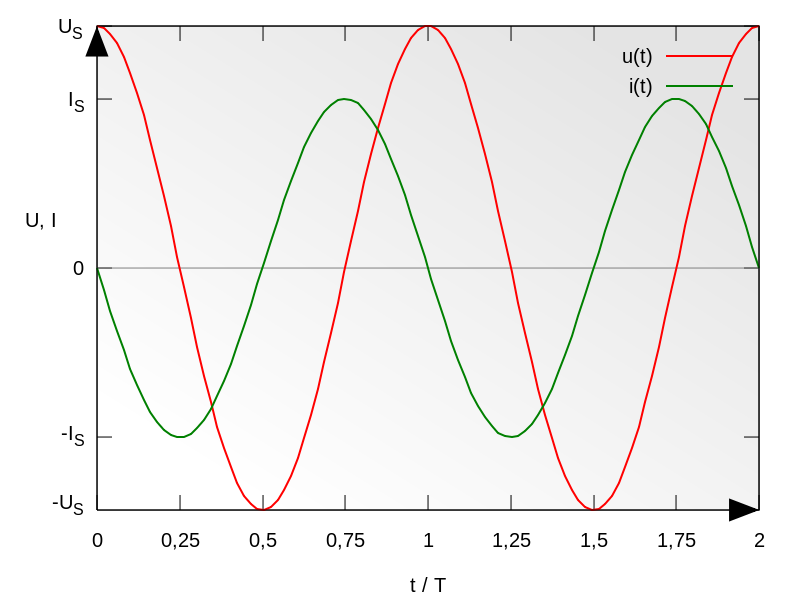
\includegraphics[width=1\textwidth,height=.75\textheight,keepaspectratio]{e05/Sinus_Voltage_and_Current_of_a_Capacitor.png}
      \attribcaption{Sinusspannung und Strom eines Kondensators}{Fabian R}{https://de.wikipedia.org/wiki/Datei:Sinus_Voltage_and_Current_of_a_Capacitor.svg}{\ccbysa}
    \end{figure}
    \column{0.63\textwidth}
    {\small
    \begin{block}{}
      \begin{description}
        \item[$t=0$] Kondensator ist geladen; es fließt kein Strom
        \item[$0<t<0,25$] Kondensator wird entladen; der Stromfluss nimmt zu
        \item[$t=0,25$] Kondensator ist entladen; der Stromfluss ist am Maximum
        \item[$0,25<t<0,5$] Kondensator wird umgekehrt aufgeladen; der Stromfluss in diese Richtung nimmt ab
        \item[$t=0,5$] Kondensator ist umgekehrt aufgeladen; es fließt kein Strom
      \end{description}
    \end{block}
    }
  \end{columns}
\end{frame}

\begin{frame}
  \frametitle{Eselsbrücke}
  \begin{block}{Merksatz}
    Kondensator: Strom eilt vor
  \end{block}
\end{frame}

\begin{frame}
  \frametitle{Kapazitiver Widerstand}

  Abhängig von der Frequenz $f$.

  \begin{block}{Impedanz als Scheinwiderstand}
    \huge{$X_C = \frac{1}{2 \cdot \pi \cdot f \cdot C}$}
  \end{block}

  \pause
  Der Scheinwiderstand sinkt bei zunehmender Frequenz.\\
  Der Scheinwiderstand sinkt bei größerer Kapazität.
\end{frame}

\begin{frame}
  \begin{center}
    \begin{tabular}{l||p{.8\textwidth}}\hline
      \textbf{TC208} & \textbf{Mit zunehmender Frequenz...}\\ \hline\hline
      A & steigt der Wechselstromwiderstand des Kondensators. \\ \hline
      B \only<2>\checkmark & sinkt der Wechselstromwiderstand des Kondensators. \\ \hline
      C & steigt der Wechselstromwiderstand des Kondensators bis zu einem Maximum und sinkt dann wieder. \\ \hline
      D & sinkt der Wechselstromwiderstand des Kondensators bis zu einem Minimum und steigt dann wieder. \\ \hline
    \end{tabular}
  \end{center}
\end{frame}


\section*{Schaltungsarten}

\subsection*{Parallel\-schaltung}

\begin{frame}
  \frametitle{Parallelschaltung von Kondensatoren}
  \begin{center}
    \begin{figure}
      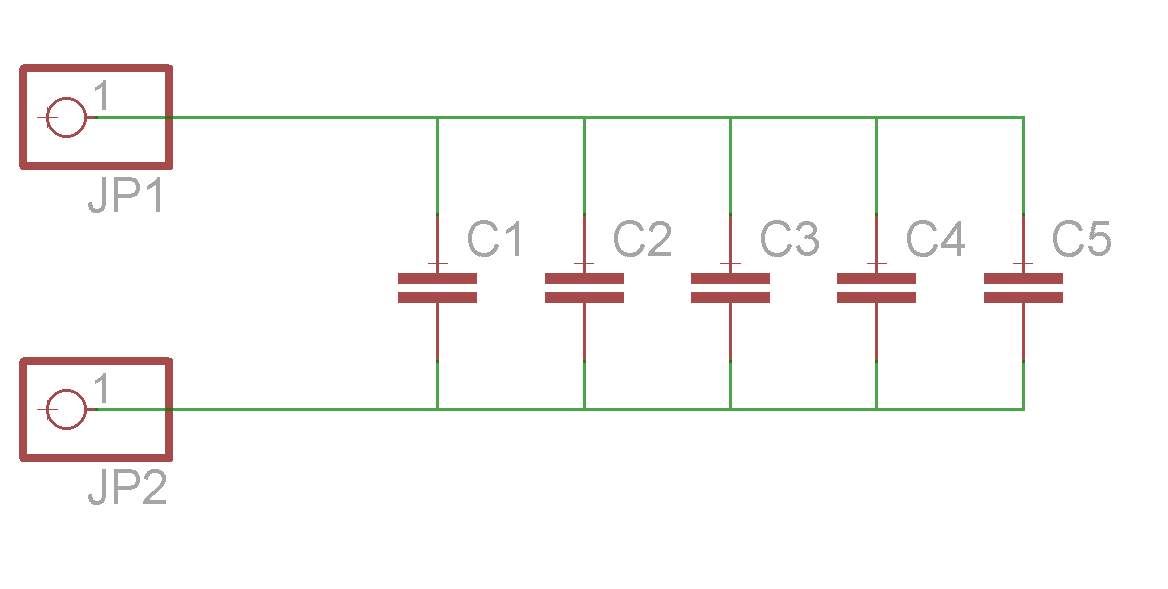
\includegraphics[width=0.7\textwidth,height=.5\textheight,keepaspectratio]{e05/c-parallel.png}
      \caption{Parallelschaltung von Kondensatoren {\tiny mit Eagle erstellt}}
    \end{figure}
  \end{center}
  \begin{block}{Parallelschaltung}
    $C_{ges} = C_1 + C_2 + C_3 + C_4 + C_5$
  \end{block}
\end{frame}

\begin{frame}
  \begin{exampleblock}{TC206}
    Drei Kondensatoren mit den Kapazitäten $C_{1} = 0,1 \mu F, C_{2} = 150 nF$ und $C_{3} = 50000 pF$ werden parallel geschaltet. Wie groß ist die Gesamtkapazität?
  \end{exampleblock}
  \pause
  \begin{center}
    $C_{ges} = C_1 + C_2 + C_3 = 0,1 \mu F + 150 nF + 50000 pF = 0,3 \mu F$
  \end{center}
\end{frame}

\subsection*{Reihen\-schaltung}

\begin{frame}
  \frametitle{Reihenschaltung von Kondensatoren}
  \begin{center}
    \begin{figure}
      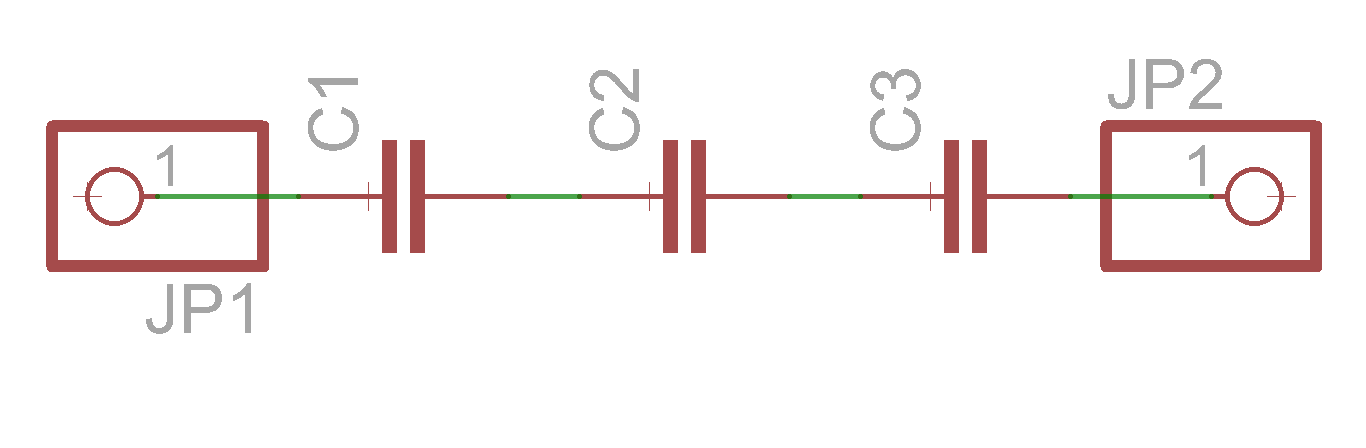
\includegraphics[width=0.6\textwidth,height=.5\textheight,keepaspectratio]{e05/c-reihe.png}
      \caption{Reihenschaltung von Kondensatoren {\tiny mit Eagle erstellt}}
    \end{figure}
  \end{center}
  \begin{block}{Reihenschaltung}
    $\frac{1}{C_{ges}} = \frac{1}{C_1} + \frac{1}{C_2} + \frac{1}{C_3} + \frac{1}{C_4} + \frac{1}{C_5}$\\
    $C_{ges} = \cfrac{1}{\frac{1}{C_1} + \frac{1}{C_2} + \frac{1}{C_3} + \frac{1}{C_4} + \frac{1}{C_5}}$
  \end{block}
\end{frame}

\begin{frame}
  \begin{exampleblock}{Reihenschaltung}
    Zwei Kondensatoren von $100 pF$ und $150 pF$ sind hintereinander (in Serie) geschaltet. Berechnen Sie die Gesamtkapazität.
  \end{exampleblock}
  \pause
  \begin{center}
    $C_{ges} = C_1 \parallel C_2 = 100 pF \parallel 150 pF = \cfrac{1}{\frac{1}{100 pF} + \frac{1}{150 pF}} = 60 pF$
  \end{center}
\end{frame}

\begin{frame}
  \frametitle{Kennzeichnung von Kondensatoren}
  \begin{itemize}
    \item ähnlich wie bei SMD-Widerständen
    \item Größenkennzeichnung (Milli (m), Mikro ($\mu$), Nano (n), Piko (p)) an die Stelle des Kommas
    \item Beispiel: 4n7
  \end{itemize}
\end{frame}

\begin{frame}
  \begin{alertblock}{fakultative Hausaufgaben}
    Aus Fragenkatalog Klasse E Fragen TB610--TB613.\\
    Aus Fragenkatalog Klasse E Kapitel 1.3.2 Kondensator (Fragen TC201--TC208).
  \end{alertblock}
\end{frame}



\renewcommand{\refname}{Referenzen}

\hypertarget{refs}{}
\textcolor{white}{} \\ %\vspace{} geht nicht
\Large Referenzen/Links
\footnotesize

\begin{thebibliography}{}
  \bibitem{e03}   Moltrecht E 05: \\
    \url{https://www.darc.de/der-club/referate/ajw/lehrgang-te/e05/}
  \bibitem{wp}    Wikipedia DE: \\
    \url{http://de.wikipedia.org/wiki/Kondensator_(Elektrotechnik)}\\
\end{thebibliography}

% Hier könnte noch eine Kontaktfolie stehen

\end{document}

